\documentclass{sig-alternate}

\usepackage{color}
\usepackage{url}

\begin{document}
\conferenceinfo{OZCHI}{'14, Dec 2-5, 2014, Sydney, Australia}

\title{Visualising a Live Coding Arts Process}

\numberofauthors{3} 
\author{
\alignauthor Arrian Purcell\\
       \affaddr{Australian National University}\\
       \affaddr{Canberra, ACT, Australia}\\
       \email{u5015666@anu.edu.au}
\alignauthor Henry Gardner\\
       \affaddr{Australian National University}\\
       \affaddr{Canberra, ACT, Australia}\\
       \email{henry.gardner@anu.edu.au}
\alignauthor Ben Swift\\
       \affaddr{Australian National University}\\
       \affaddr{Canberra, ACT, Australia}\\
       \email{ben.swift@anu.edu.au}
}

\maketitle
\begin{abstract}

We have considered software visualisations as a means of communicating the real-time programming process of a ``live coding'' computer-music performance. Following a field study at a festival of the contemporary arts, two sets of complementary, interaction-driven visualisations were developed and incorporated into a live coding system. A formal audience experiment was then undertaken to compare these visualisations and to survey their contributions to the audience experience, with emphasis on the two axes of ``understanding'' and ``enjoyment''. The reactions of the live coding performer (the programmer) were also evaluated in a process of video-cued recall.

The visualisations examined in the formal audience experiment appeared to positively contribute to enjoyment. Although the results also demonstrated the potential for visualisation to communicate the live coding performer's intention to an audience, their impact on ``understanding'' did not seem to be sustained for the duration of a performance as well as they might. In addition, there remains an ongoing challenge to match the audience's mental model with that of the programmer.

\end{abstract}

\category{H.5}{Information Interfaces and Presentation}{Miscellaneous}

% \terms{Theory}

\keywords{live coding, software visualisation}

\section{Introduction}

``Show us your screens ... Code should be seen as well as heard'', says the draft manifesto of the international organisation ``TOPLAP'' \cite{Toplap} which is devoted to the decade-old arts performance practice ``live coding''. Live coding is a performance practice where computer code is created in front of a live audience to generate computer music, video and visualisations in real time. The ``show us your screens'' exhortation underscores the need for authenticity to distinguish this artform from aligned performance art genres such as VJ'ing. 

Live computer music is the primary product of live coding. Where they exist, live coded graphics and video are launched and orchestrated directly by commands from the computer keyboard for artistic impact. Commonly, non-expert live coding audience members spend much of their time staring at raw computer code (text-based or visual programming languages) and, until now, no formal study has ever been undertaken to gauge an audience's understanding of that computer code and whether, from an audience perspective, code really should be ``seen as well as heard''.

Many traditional approaches to visualising code focus solely on historic source code changes, the behaviour of algorithms or the structure of the source code rather than the {\it process of programming} \cite{Novais2013}. Furthermore, within the space of  artistic live coding most of the academic treatment of visualisations have adopted a design or survey approach \cite{McLean2010b,Magnusson2013} and have not subjected alternatives to rigorous evaluation.

In this paper, we set out to evaluate the audience reception to the display of code during live coding performances and to see whether code-driven visualisations might improve both the audience enjoyment and the audience understanding of the process of a live coding performance.

\section{Field Study}

On one evening of the (name withheld for blind reviewing) arts festival in (withheld), a survey was presented to the audience of a live coding computer-music performance. The survey was designed to gain an impression of the audience response to the performance and to the projection of the computer code (a Scheme type of language with syntax highlighting). Alongside demographic and open-ended questions, audience members were solicited to indicate which of a number of curves best represented their personal ``enjoyment'' and ``understanding'' of the performer's actions in typing the computer code through the performance. These curves were analysed based on their binning into ``high", ``medium", and ``low'' categories for the ``beginning'', ``middle'' and ``end'' of the performance. Other survey questions addressed the sense of ``liveness'' of the performance \cite{Auslander} and whether the code-projections were found to be confusing.

Of the 13 survey respondences received, 6 indicated a high level of enjoyment throughout the whole performance with the remaining 7 responses mostly indicating alternating levels of enjoyment. No responses indicated a low level of enjoyment throughout the performance.

Only 2 of the 13 respondents indicated that they understood the relationship between the code projections and the music throughout the performance. Although a Chi-square analysis revealed no statistical significance between ``enjoyment'' and ``understanding'' per se, it was remarkable that 3 of the 6 respondents who indicated a high level of enjoyment throughout the performance, also indicated a pattern of their understanding increasing from low to high as the performance progressed. Nine of the 13 respondents stated that the code projections provided a sense of liveness to the performance and the remainder stated that these visuals had no effect on their sense of liveness. Four respondents felt that the code projections were confusing, 5 stated that they were not, and 4 did not answer the question.

Taken as a whole, the results of this small field study were salutatory for the notion of ``seeing as well as hearing'' code during a live coding performance, especially as far as the general public is concerned. The best that can be said for the code projections is that a majority of the audience felt that they made the performance seem more ``live''. However a minority stated that they found the projections confusing and only a very small number of respondents claimed to have actually understood what the programmer was doing. We were quite intrigued by the small cohort of respondents whose understanding increased through the performance and whose ejoyment remained high, and we wished to test whether augmenting code projections with additional visualistions might increase this pattern of understanding, and enjoyment across an audience. 

\section{Design}

\begin{figure}
\centering
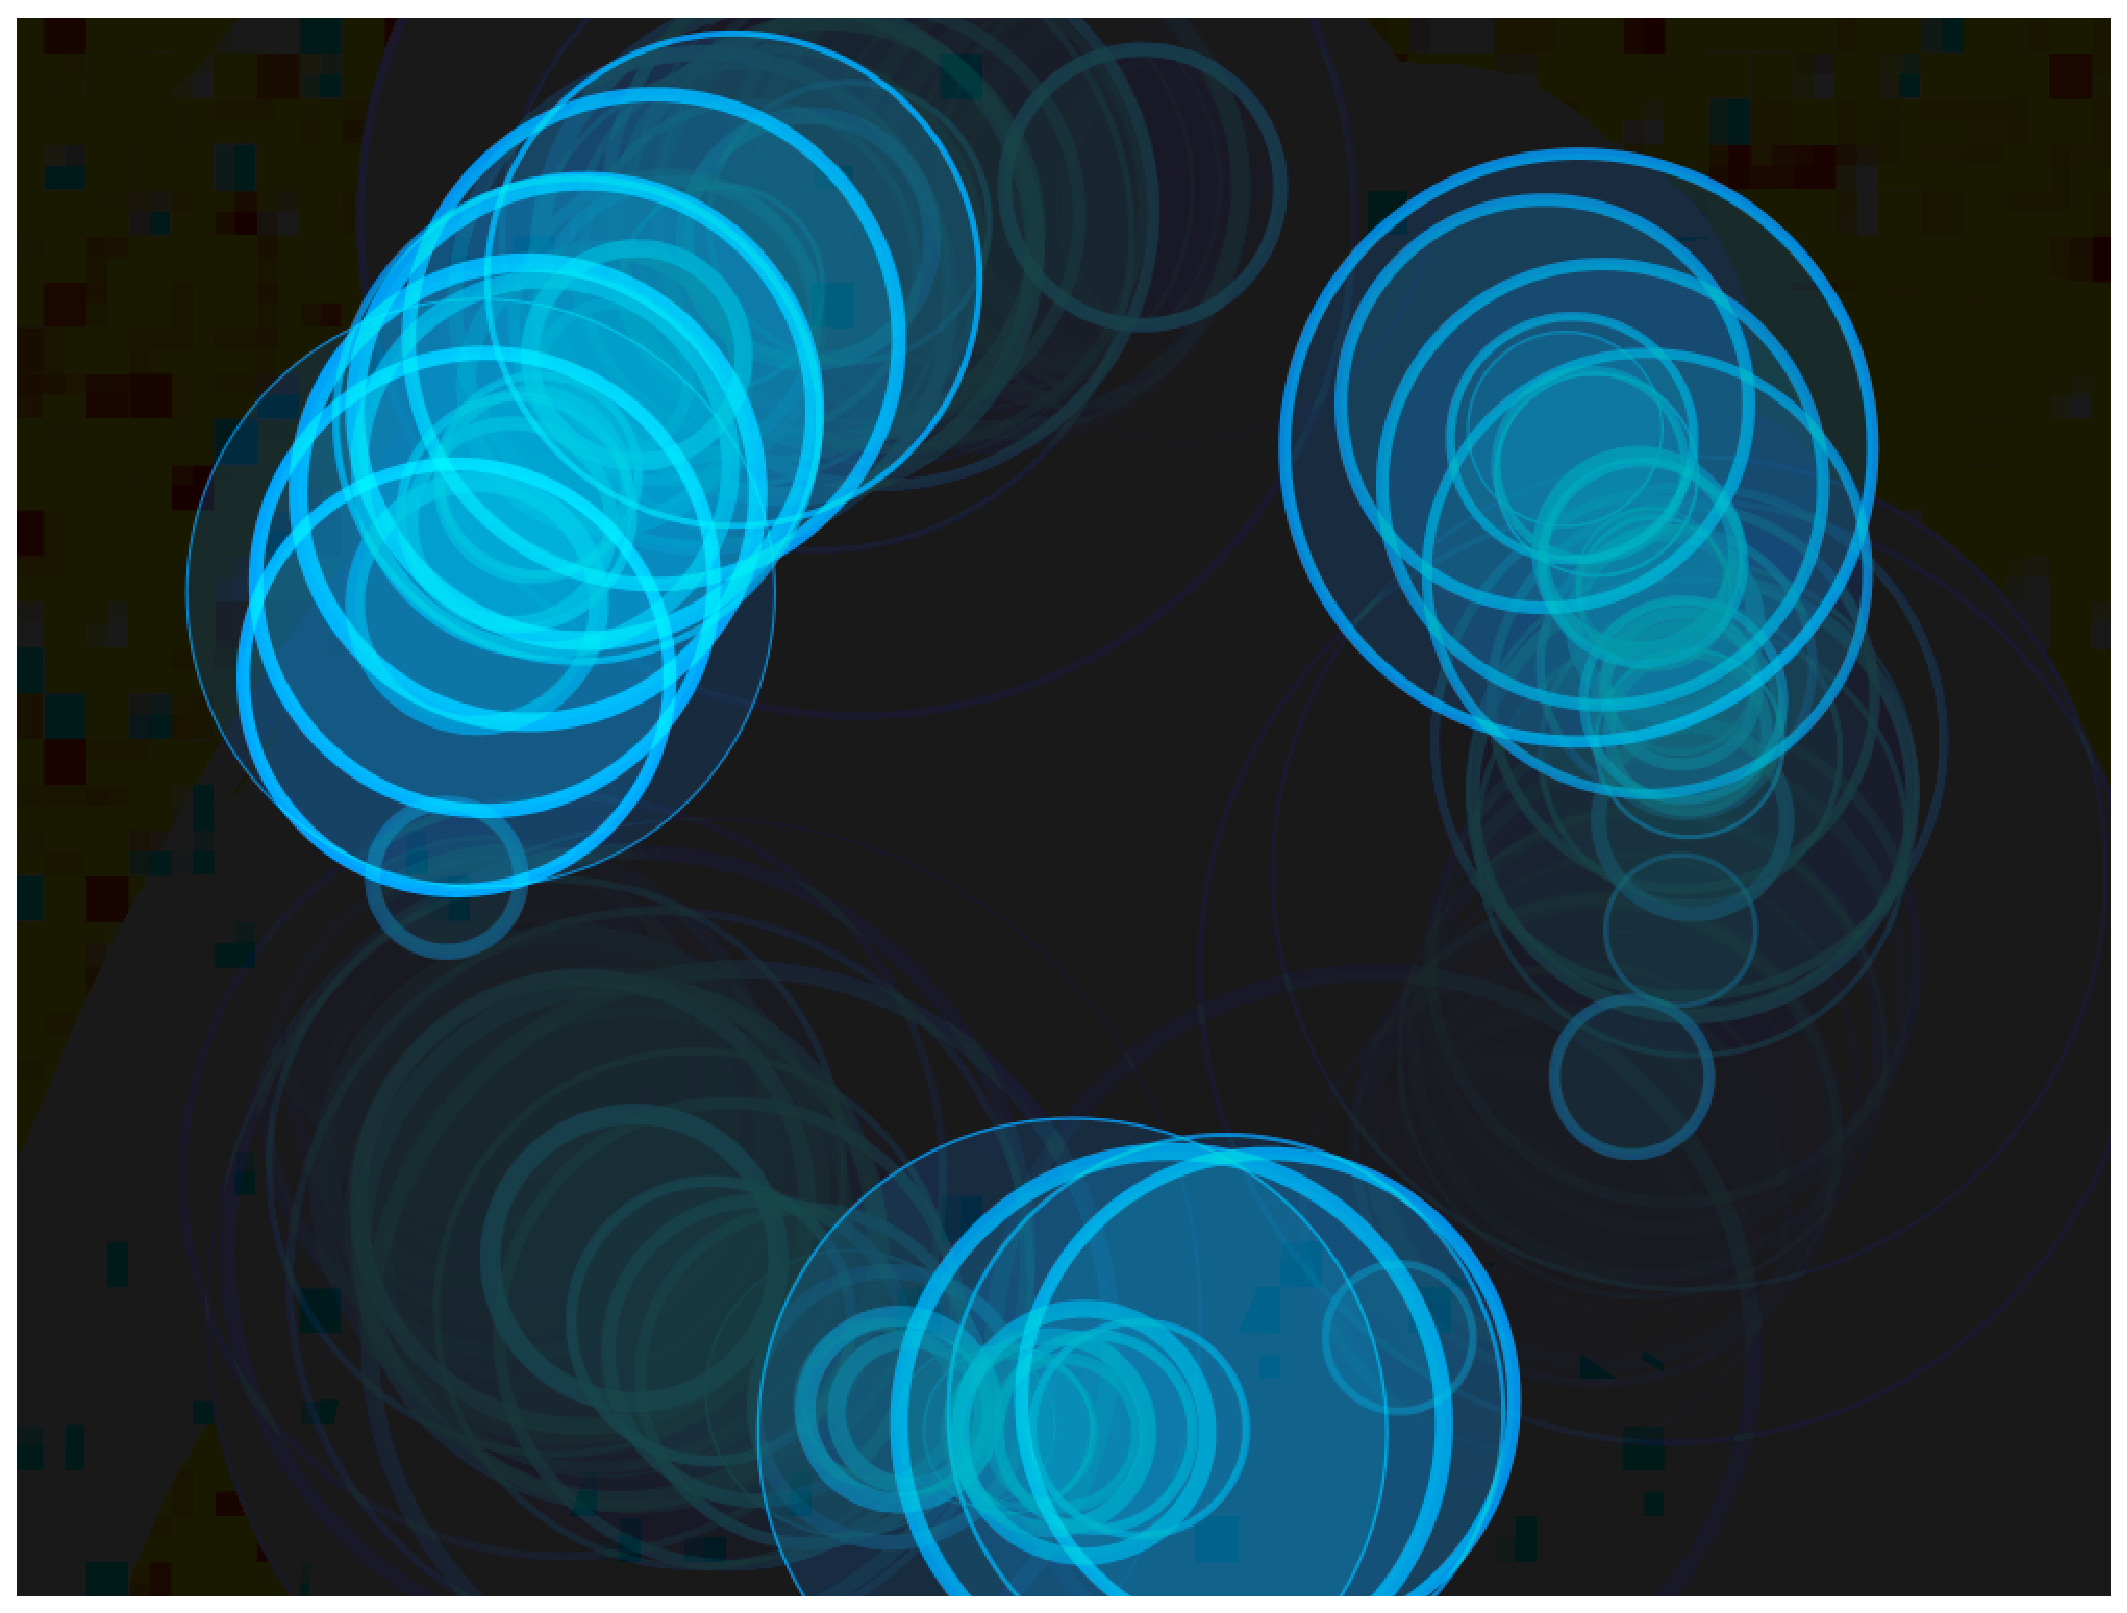
\epsfig{file=aesthetic-vis.eps, width=3.4in}
\caption{Example aesthetic visualisation.}
\label{fig:aesthetic-visualisation}
\end{figure}

\begin{figure}
\centering
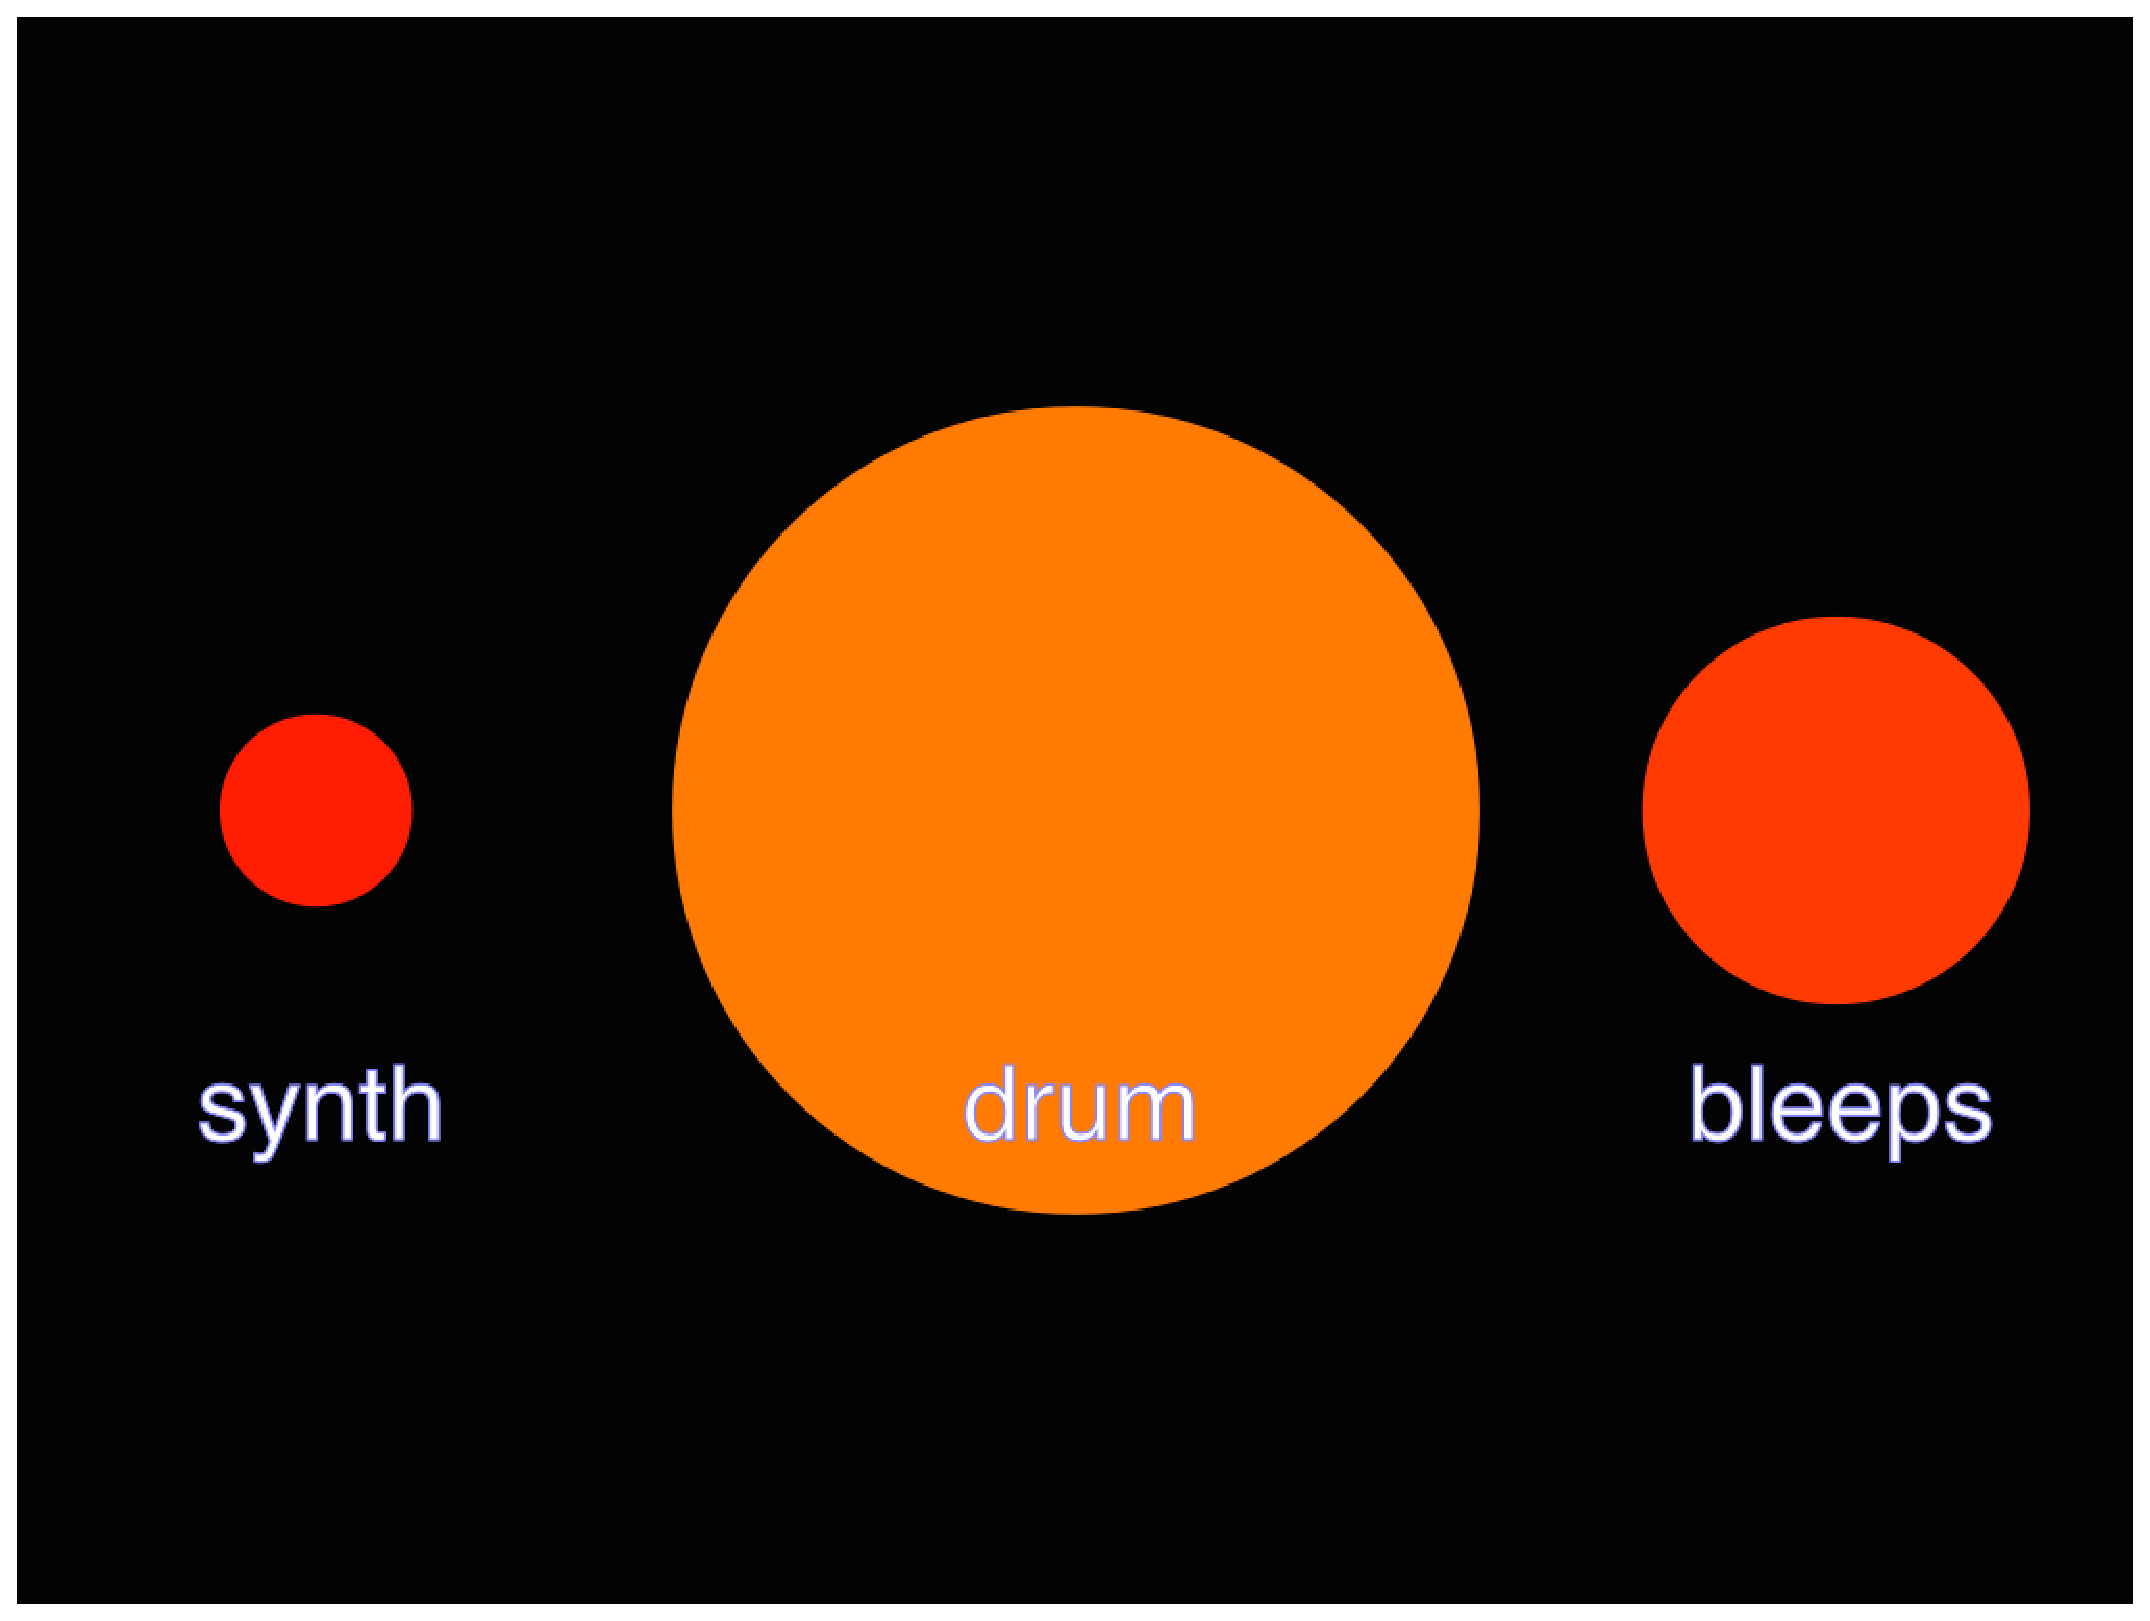
\epsfig{file=didactic-vis.eps, width=3.4in}
\caption{Example didactic visualisation.}
\label{fig:didactic-visualisation}
\end{figure}

Two sets of visualisations were developed based on the results of the initial survey and the literature. The first set focussed on increasing audience retention and user experience by maximising aesthetic appeal \cite{Cawthon2007} while communicating the actions of the programmer. The second set attempted to communicate program behaviour and visualise output while communicating the actions of the programmer. These two approaches will be referred to as the ``aesthetic'' condition and the ``didactic'' condition respectively.

The set of didactic visualisations predominantly focussed on the relationship between the live coding active processes and their behaviour. The visualisations prominently displaying the names of the active functions with visual indication of the number of functions running and their callback time. Bright colours and solid shapes were used to ensure constant visibility and communicate the intention of the underlying code. Overall, four visualisations were presented with each introduced depending on the number of active functions. It was predicted that taking a more educational approach would see a reduction in audience confusion through the performance.

The set of aesthetic visualisations focussed less on the programmatic aspects of the live coding performance, rather intending to provide additional visual interest to the projected code thereby prolonging attention. More variety was used in visual structure and colour. Again, four visualisations were presented, varying the visualisation based on the number of active functions. It was predicted that focussing on the aesthetic nature of the visualisations would assist in audience retention and result in a consistency of interest through the performance.

\section{User Study}

Visualisations were presented to an audience alongside code during a live coding performance and surveys were distributed. The performance was run as two ten minute improvised songs with each song demonstrating one of the two experimental visualisation conditions, either the didactic condition or the aesthetic condition. The experiment was run twice, with two separate participant groups, swapping the order in which the two sets of visualisations were presented to the audience.

The audience members completed a survey consisting of four sections over the course of the performance. These sections included a demographic information section, opinion of the first visualisation, opinion of the second visualisation and a section investigating the audience's overall opinion of the performance. The sections regarding the visualisations predominantly focussed on the enjoyment and understanding related to the visualisation while the final section focussed on eliciting potential improvements.

Following an explanation of the structure of the experiment and allowing the participants to complete the initial demographic section of a survey, the live coder began the first performance utilising one of the two visualisations. Following this first set, the second section of the survey was completed. A second set was then played using the alternative visualisation. Following this second set, the same survey questions were administered again, again asking the participants specifics about their enjoyment and understanding related to the specific visualisation demonstrated. A final survey question was then asked relating to their opinion regarding the whole performance and their suggested improvements.

To further inform the outcomes of the experiment a video-cued recall interview was conducted with the live coder following the performance. One performance was examined critically and comparisons were drawn between the live coder's enjoyment and understanding and the audience's enjoyment and understanding.

\subsection{Results}

A total of 41 responses were received with roughly equal split of 19 and 22 participants in each group. $66\%$ were male and $76\%$ were aged between 18 and 32. $78\%$ of the participants had not seen a live coding performance before.

Enjoyment and understanding were evaluated against the aesthetic and didactic visualisations. Results and statistical analysis of the differences between the aesthetic and didactic conditions follows. A significance level of $0.05$ was used with the chi-squared test for independence.

\subsubsection{Enjoyment}

\begin{figure}
\centering
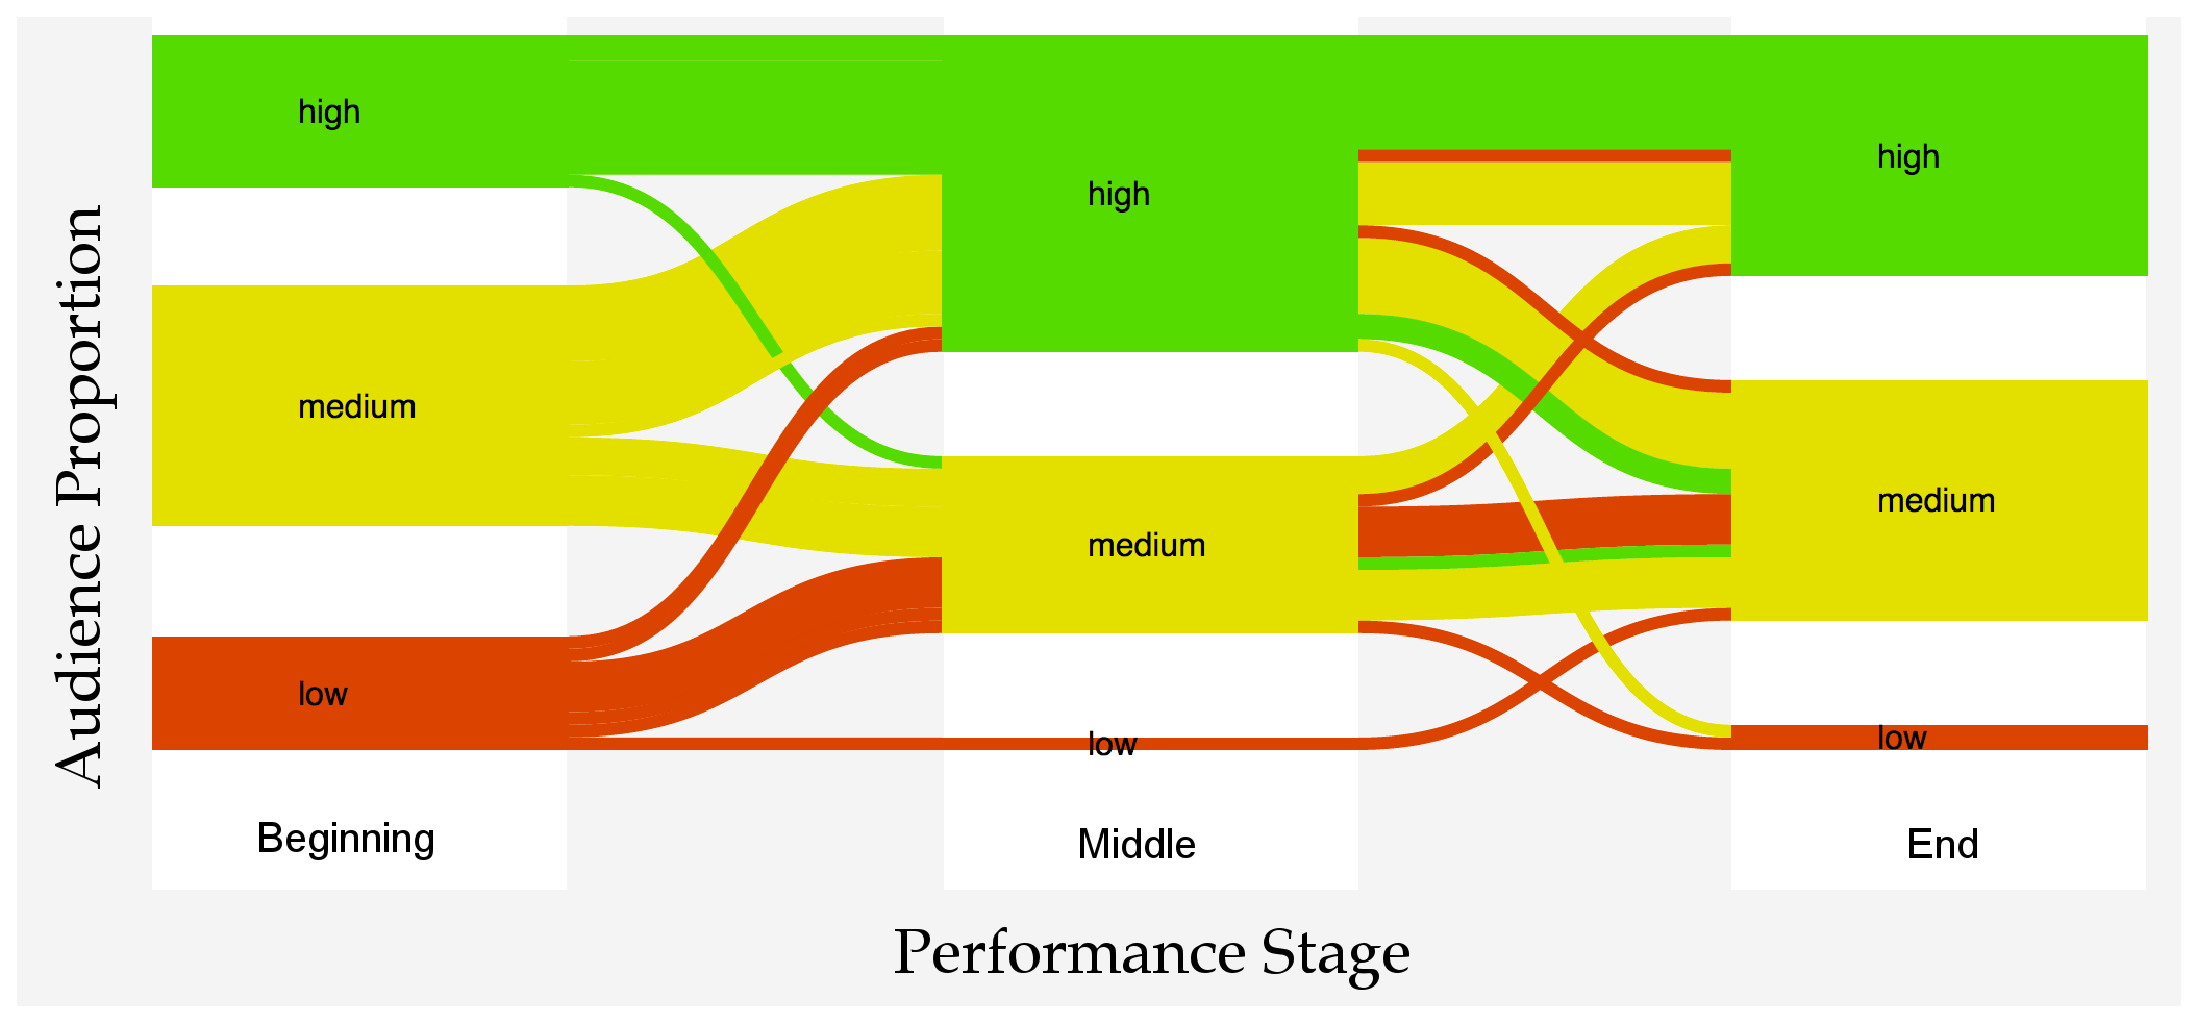
\epsfig{file=aesthetic-enjoyment-final.eps, width=3.4in}
\caption{Audience reported enjoyment during the beginning, middle and end of the performance with the ``aesthetic'' condition.}
\label{fig:aesthetic-enjoyment}
\end{figure}

\begin{figure}
\centering
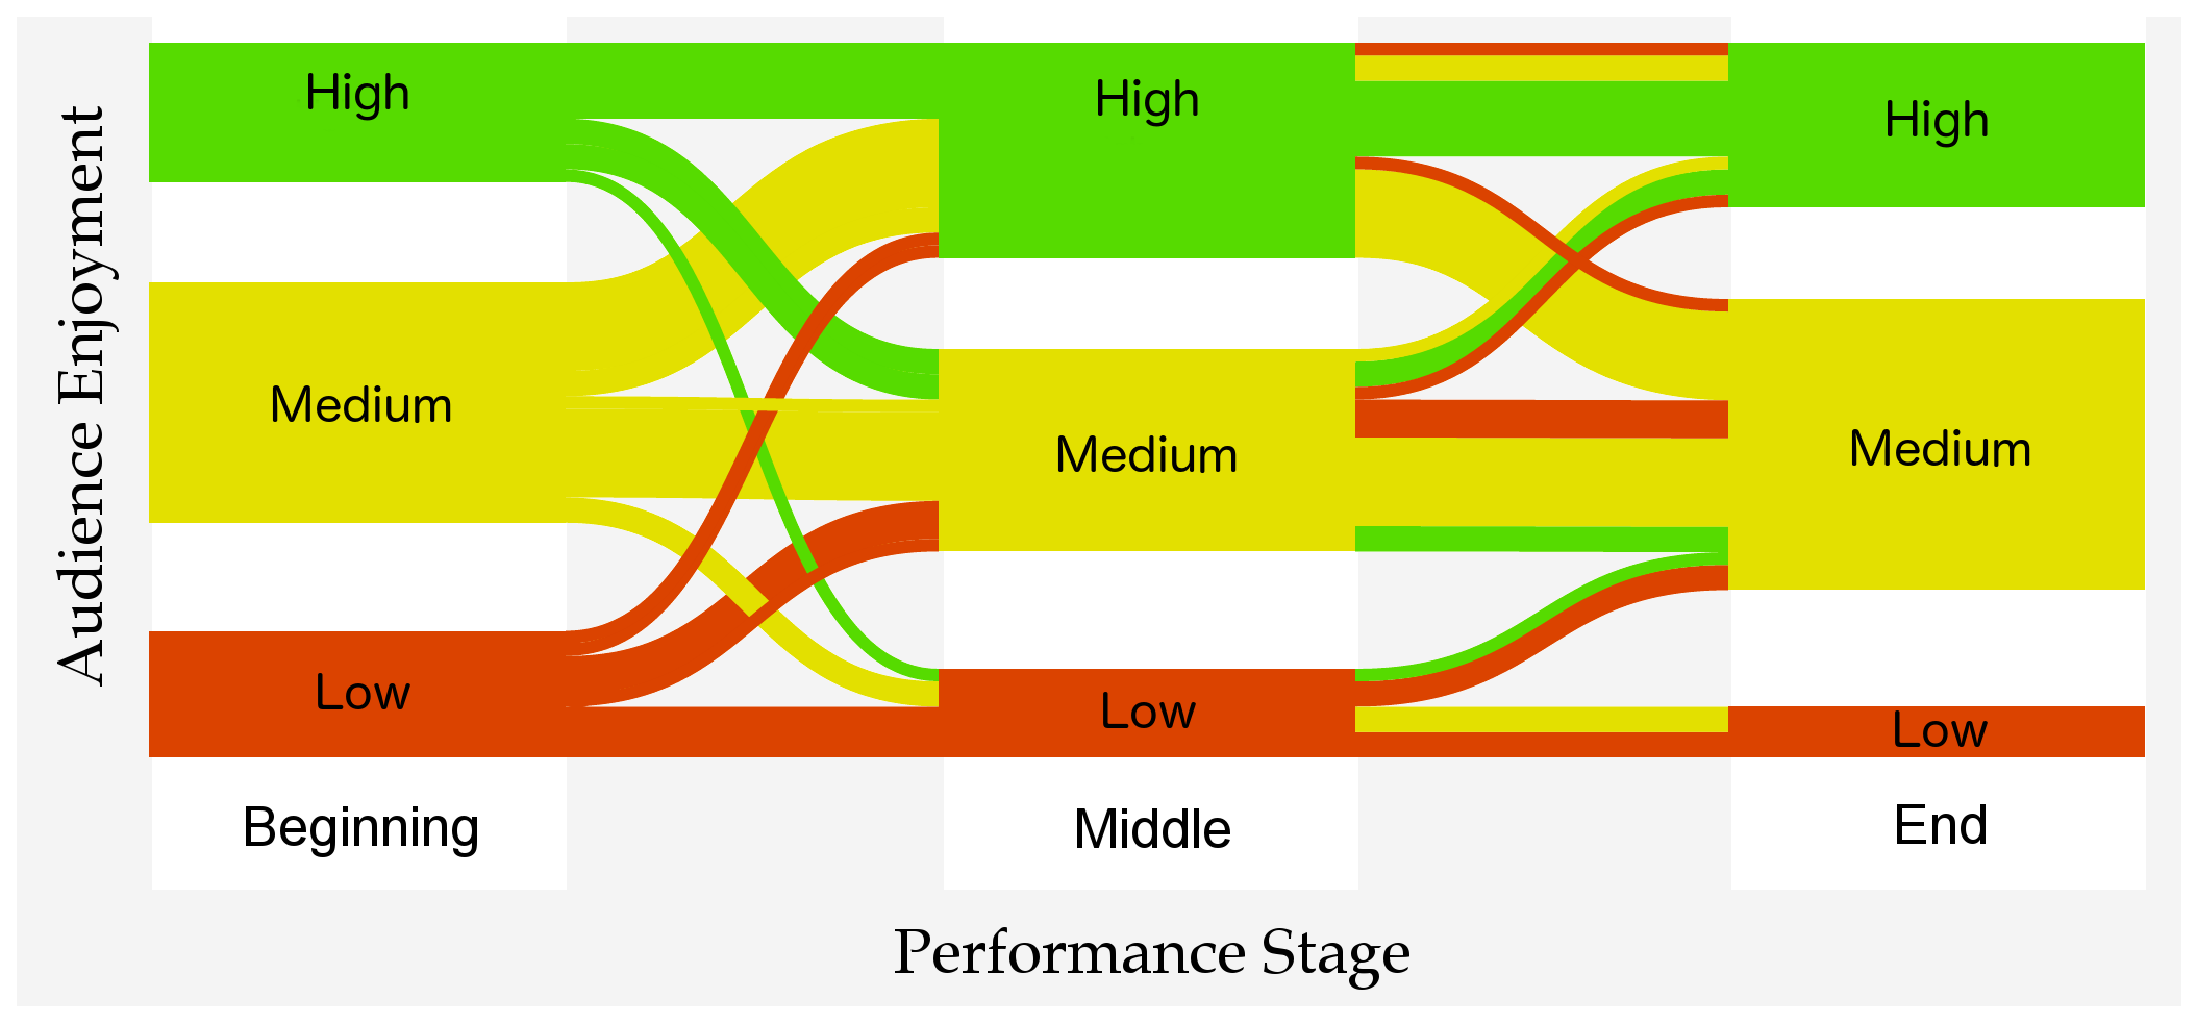
\epsfig{file=didactic-enjoyment-final.eps, width=3.4in}
\caption{Audience reported enjoyment during the beginning, middle and end of the performance with the ``didactic'' condition.}
\label{fig:didactic-enjoyment}
\end{figure}

Overall, a large proportion ($> 50\%$) of the participants stated that both visualisations helped their enjoyment of the performance. $76\%$ stated that the aesthetic visualisations helped their enjoyment compared to $56\%$ of the participants that stated the didactic visualisations helped their enjoyment. No significant difference between the two visualisations' effect on enjoyment was found ($\chi^2=3.7733,df=2,p=0.1516$).

Participants were asked to rate their enjoyment during the beginning, middle and end of the performance (see Figure~\ref{fig:aesthetic-enjoyment} and Figure~\ref{fig:didactic-enjoyment}). During the didactic performance, $15\%$ of the audience stated that enjoyment increased during the beginning and was steady for the remainder whereas $24\%$ of the audience said the same during the aesthetic performance. Approximately $30\%$ of the audience during both the aesthetic and didactic performances stated that their enjoyment remained steady throughout.

\subsubsection{Understanding}

\begin{figure}
\centering
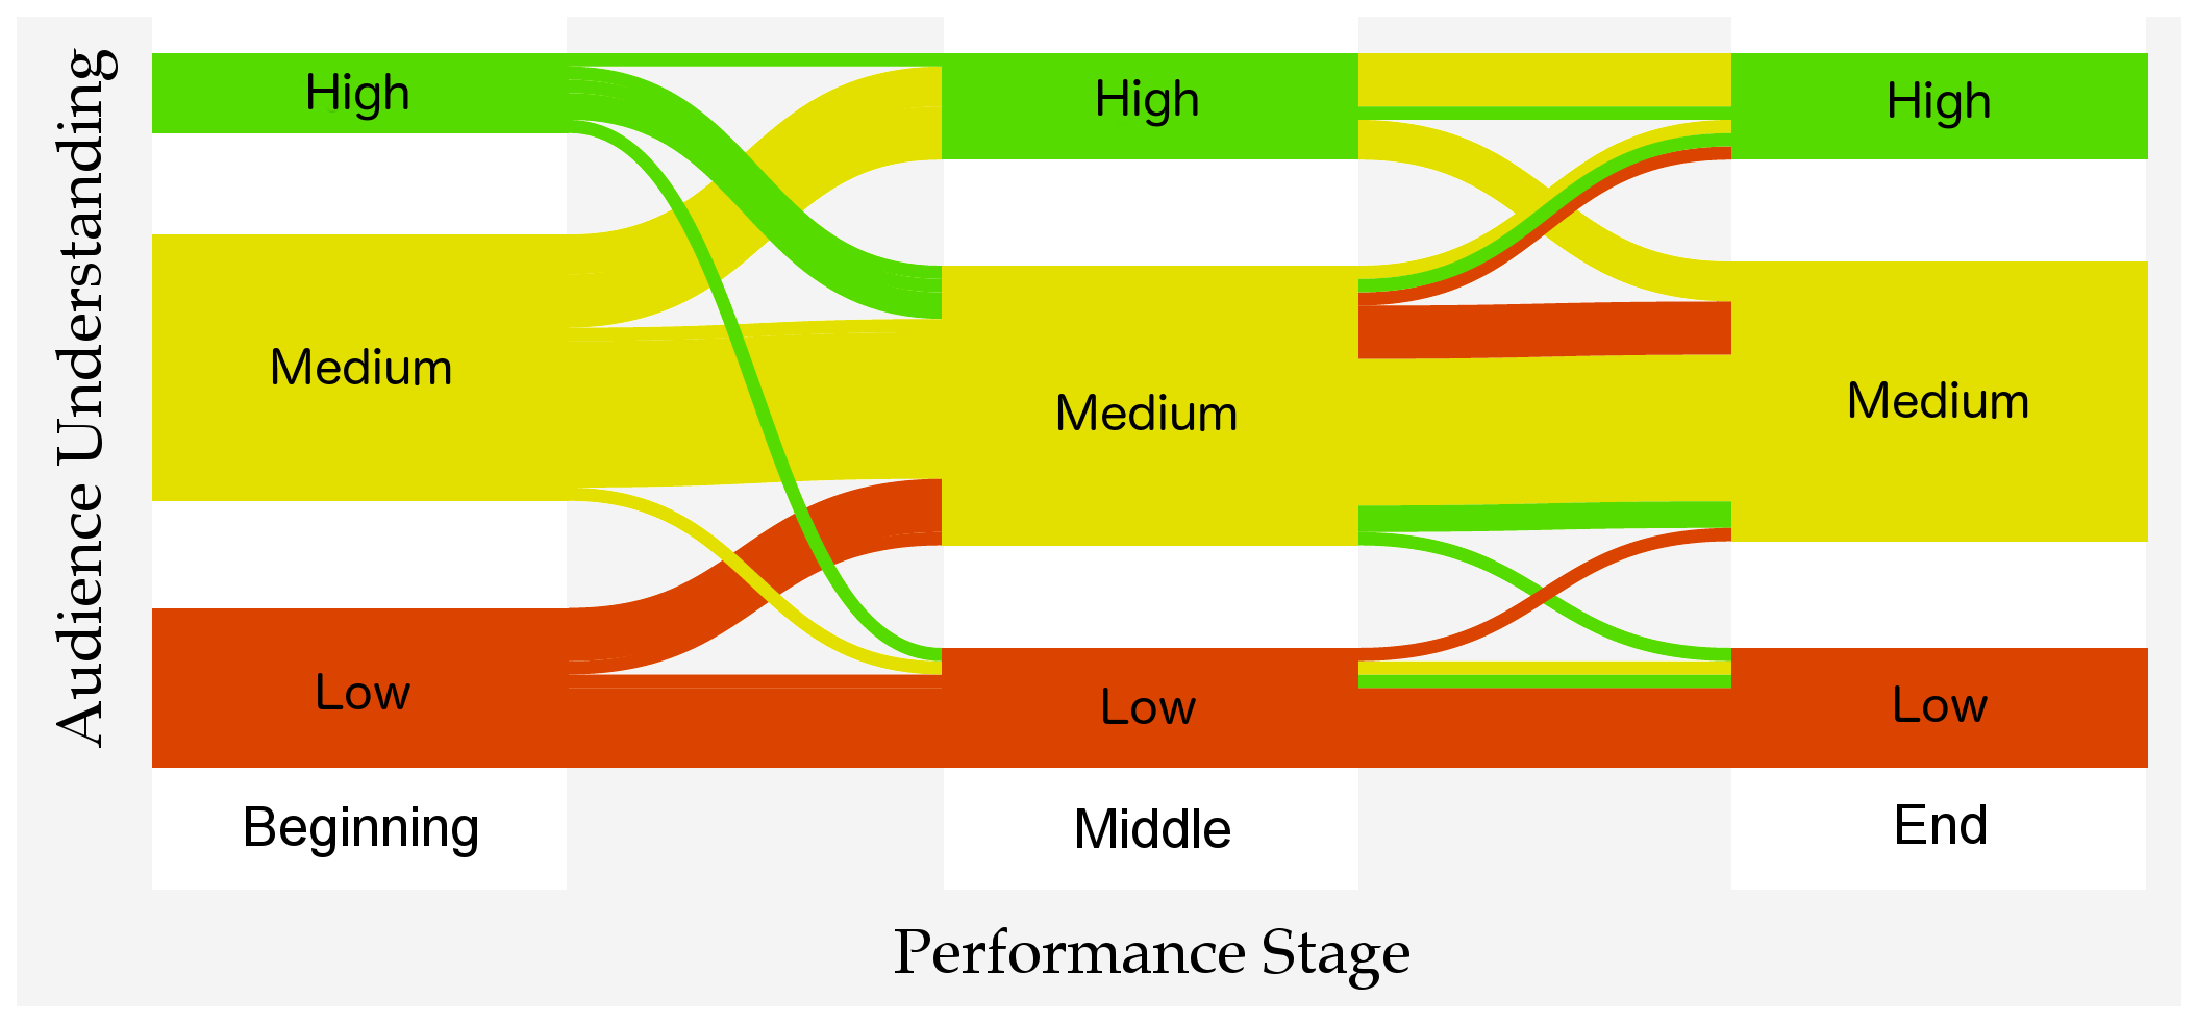
\epsfig{file=aesthetic-understanding-final.eps, width=3.4in}
\caption{Audience reported understanding during the beginning, middle and end of the performance with the ``aesthetic'' condition. Line width indicates proportion of the audience. Link colour between the performance stages indicates the understanding level at the beginning of the performance.}
\label{fig:aesthetic-understanding}
\end{figure}

\begin{figure}
\centering
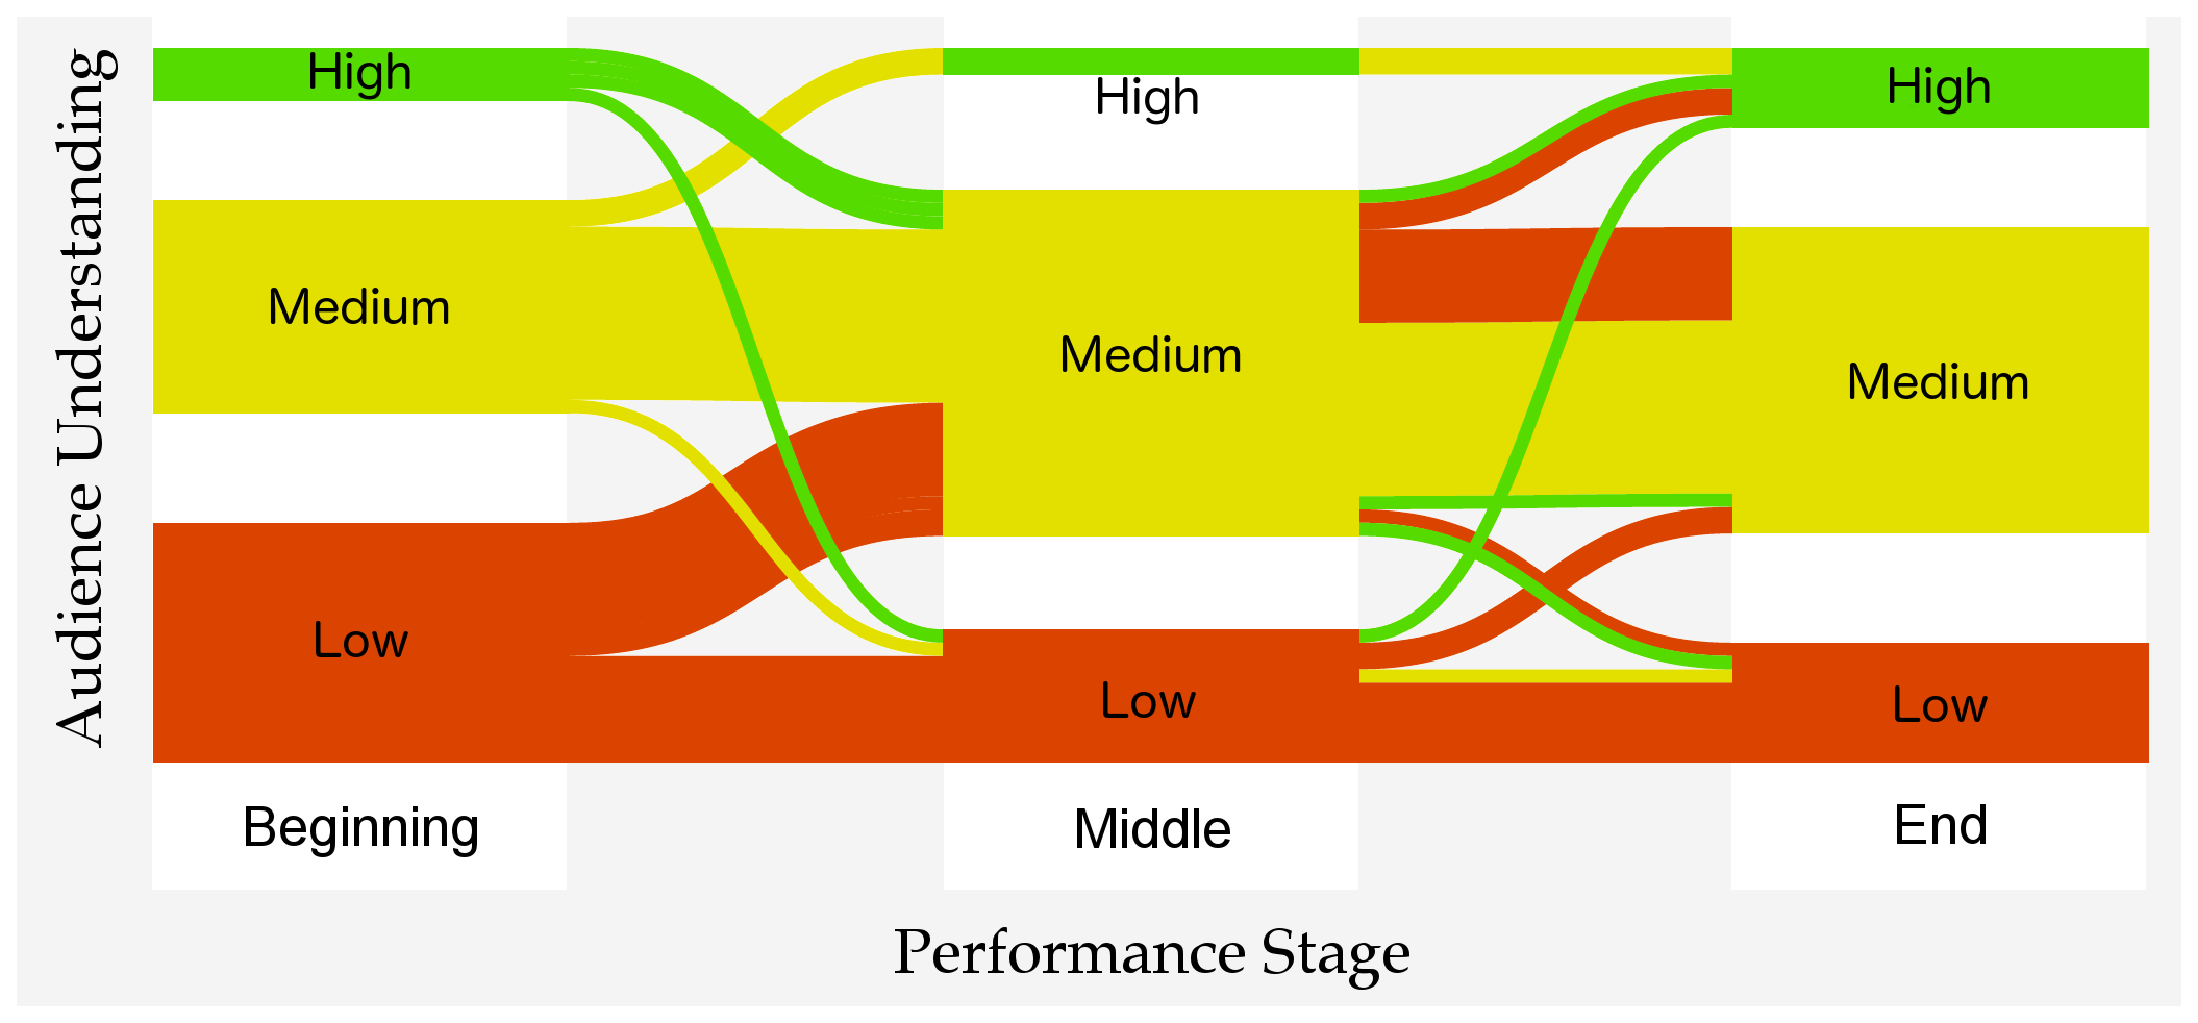
\epsfig{file=didactic-understanding-final.eps, width=3.4in}
\caption{Audience reported understanding during the beginning, middle and end of the performance with the ``didactic'' condition.}
\label{fig:didactic-understanding}
\end{figure}

Overall, $37\%$ participants stated specifically that the didactic visualisations helped them to understand the code, whereas $12\%$ participants stated that the aesthetic visualisations assisted in understanding the code. A significant difference between the visualisations effect on understanding was found ($\chi^2=7.1986,df=2,p=0.02734$).

Participants were asked to rate their understanding during the beginning, middle and end of the performance (see Figure~\ref{fig:aesthetic-understanding} and Figure~\ref{fig:didactic-understanding}). During the didactic and aesthetic performances, $49\%$ and $44\%$ of the participants respectively stated that their understanding remained the same throughout the performance. During the didactic performance, $10\%$ of the audience had an understanding that tended downwards (eg. high to low) compared to $20\%$ of the audience during the aesthetic performance. However, this gain was offset by the audience understanding at the beginning of the performance in which $44\%$ of the audience indicated low understanding with the didactic visualisations compared to $30\%$ with the aesthetic visualisations.

% \subsubsection{Liveness}

% Participants were asked to discuss how each visualisation influenced or impacted the liveness of the performance. Concepts identified included positive and negative valence towards the didactic visualisations, positive and negative valence towards the aesthetic visualisations and the relevance of visual source code. 

% within the discussion included the positive and negative aspects of the didactic visualisations, the positive and negative aspects of the aesthetic visualisations, source code discussion and statements indicating an understanding between the visuals and the source code.

% Overall, $54\%$ of the audience indicated negative valence towards the didactic visualisation regarding liveness referencing a variety of reasons including that the ``visuals only responded to what was typed'', that the ``musical forms didn't occur at the most expected times'' and that the visualisations ``perhaps made the performance seem too polished''.

% On the other hand, $34\%$ of the audience indicated positive valence towards the didactic visualisations suggesting that ``it was easier to follow this visualisation than the code'', ``the visualisations clearly showed the changes being made to the code'' and that these visualisations ``helped more with communicating that the performance was live''.

% $40\%$ of the audience had negative valence towards the aesthetic visualisation its effect on the sense of liveness. Reasons cited include that the ``influence is not clear'' between the code and the visuals, that ``the visualisation did not make much sense'' and that the ``visualisations did nothing to suggest that the performance was live''.

% $32\%$ had positive valence towards the aesthetic visualisation. A variety of the response included that these visuals were ``less dominating and more complementary'' and that ``the visualisations helped to show when a piece of code started working''.

% A relatively large proportion ($28\%$) of the audience discussed the importance of the source code to the sense of liveness of the performance such as that the ``code showed what the musician was doing physically''. A further $5\%$ of the audience demonstrated a deeper understanding of the live coding process such as ``changing values produced changes in tone and speed of the music pitch''.

\subsection{Discussion}

Overall enjoyment of the visualisations was high. This was the case for both the aesthetic and didactic visualisations.

The enjoyment of the aesthetic visualisation was higher and generally increased during the earlier stages of the performances suggesting that the aesthetic visualisations held the audience's attention consistently for a longer period.

The didactic visualisation had a more constant decrease in enjoyment throughout the performance. Audience suggested improvements offer some insight with some stating that the visualisations were competing with the projected code. One audience member stated that they ``found them distracting'' and that they ``preferred just to read the code''. There was indication that the didactic visualisations contributed more to audience fatigue through the performance with decreased enjoyment during the later stages of the performances compared to the aesthetic visualisations. Furthermore, features of the didactic visualisation confused the audience. For example, one audience member stated that ``it felt harder to understand the code'' during the didactic performance than the aesthetic performance.

There was indication that the experience of the live coder and the experience of the audience was fundamentally different. For example, many members of the audience stated that they drifted between focussing on the music, focussing on the visualisations and focussing on the code. However, the live coder stated in the interview that their focus was dedicated purely to the code and the music, rarely drifting. In one particular section of the interview in reference to the visualisations, the live coder stated: ``I definitely wasn't paying attention to them on the day. In fact I tuned them out as best I can because I am just trying to focus on the code''. This conflicted with some members of the audience. For example, one stated that ``you could see the code being written and the visualisations helped to show when a piece of code started working''. 

The strategy for audience members for either understanding or enjoying the performance proved to be different to that of the live coder. Regarding distractions, one audience member stated that ``the visualisations were interesting but distracting''. In comparison, when asked if the visualisations were distracting the live coder stated: ``Ah, no. In general I'm just so focussed on the code''. This difference may be due to the varying experience levels or the pressure of the situation.

\section{Conclusions}
In the first systematic studies of their type, we have identified an opportunity for real-time code visualistations to improve the audience experience in a live coding computer-music performance. With few exceptions, our survey of a live coding performance revealed a generally low to medium level of audience understanding throughout that performance, although almost half the survey respondents indicated a high level of enjoyment throughout.

Our comparison of two prototype code visulisations has indicated that some sort of ``understanding'' seems to result when an audience is subjected to a ``didactic'' code visualisation and the potential for further gains in the audience's understanding of the programming process.

Results indicate the importance of providing visuals that complement the live coding performance. Visualisations targeted at the education of the audience showed an increase in understanding throughout the performance whereas visualisations targeted at the aesthetics of the music and performance indicated audience retention and a reduced fatigue effect over the didactic visualisations.

Desirable features within both visualisations could be further utilised building on the ideas developed including reacting instantly to code changes within the visualisations and providing a more effective visualisation of the relationship of code to music. These developments will provide a baseline for future visualisations.

Marshall McLuhan stated that ``The business of art is no longer the communication of thoughts or feelings which are to be conceptually ordered, but a direct participation in an experience. The whole tendency of modern communication...is towards participation in a process, rather than apprehension of concepts.'' \cite{McLuhan} Our hope is that future development of the research described in this paper will bring audiences into the process of live coding in such a way that they can feel as though they are active (albeit virtual) collaborators of a highly skilled artist.

% (ref: Letter to Harold Adam Innis, March 14 1951. From Essential McLuhan (1995), edited by Eric McLuhan and Frank Zingrone, p. 73)

% \nocite{*} % Arrian temp

\bibliographystyle{abbrv}
\bibliography{sigproc}  % sigproc.bib
% You must have a proper ".bib" file
%  and remember to run:
% latex bibtex latex latex
% to resolve all references
%
% ACM needs 'a single self-contained file'!

%line 391%
\end{document}
